\section{Verwandte Arbeiten}

\begin{figure*}
    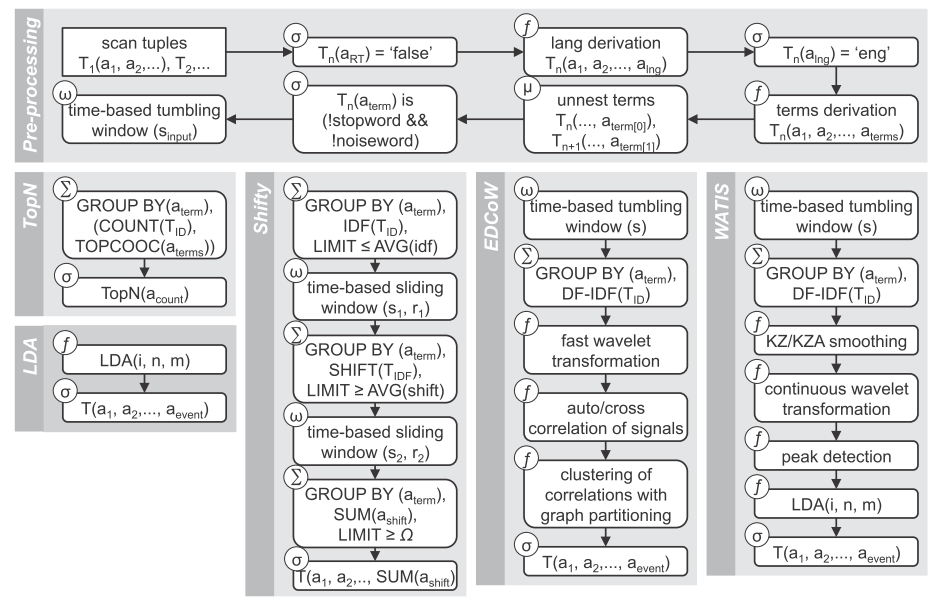
\includegraphics[width=\textwidth]{images/eventdetect.png}
    \caption{Niagarino Anfragen der fünf Erkennungs-Methoden}
    \label{fig:eventdetect}
\end{figure*}

\subsection{Event-Driven Detection}
Weiler et. al. \cite{weiler2016evaluation} evaluieren fünf State of the Art Techniken zur Erkennung von noch unbekannten Ereignissen.Niagarino wird als Implementation verwendet, eine Plattform die Apache Storm ähnelt. Die Techniken wurden als Anfragen umgesetzt, wie in \ref{fig:eventdetect} dargestellt.  Twitter-Events dienen als Datenbasis, die einem Pre-Processing gefiltert werden. Dabei werden Retweets entfernt und der Inhalt der restlichen Tweets gesäubert, es verbleiben bibliographisch erkannte englische Wörter. 

\begin{itemize}
\item TopN\\Jedem Wort wird ein Wert zugewiesen, der auf dem Inverse-Document-Frequency des Zeitfenster beruht. Nur die N-Wichtigtsten Wörter verbleiben als Event.
\item Latent Dirichlet Allocation (LDA)\\Ist ein hierarchisches Bayes-Modell, das die Variation des Vokabulars in einer Gruppe von Dokumenten bewertet. Für jedes Zeitfenster extrahiert LDA  vermutete Ereignisse, die durch Ausdrücke beschrieben werden. 
\item Shifty\\Dabei werden die Veränderungen von TopN bewertet die sich zwischen zwei Zeitfenstern ereignen.
\item Event Detection with Clustering of
Wavelet-based Signals (EDCoW)\\Der Stream wird Batches aufgeteilt, die dann per Wavelet-Analyse zu einem weiteren Event zusammengefasst werden, in dem Wörter mit erkannten Bursts stehen. Davon werden dann unwichtige Wörter entfernt. Durch Clustering erhält das Ergbnis Burst-Events die mit zwei Termen beschreiben werden.
\item The Wavelet Analysis Topic Inference Summarization
(WATIS)\\ Eine Weiterentwicklung des (EDCoW), bei dem zu jedem Burst fünf Terme geliefert werden.
\end{itemize}

\subsection{Burst Detection}
Da sich die Erkennung globaler Events mittels Esper als zumindest unvollständig erwies, wurden Methoden untersucht um das Verfahren zu Ergänzen oder zu Ersetzen.\\

Globale Events haben unter Anderem auch die Eigenschaft eine erhöhte Aktivität im Edit-Event-Stream zu verursachen. Erhöhte Aktivität (Bursts) ist ein Phänomen das bereits seit Jahrzehnten untersucht wird, daher existieren eine Reihe von Theorien und abgeleiteten Algorithmen. Dabei ist die zeitnahe Erstellung von Ergebnissen wichtig, weswegen auf eine wenig aufwändige Verarbeitung hin optimiert wird. Bursts besitzen eine Reihe an Attributen, die abhänig vom Use Case defininert werden. Dazu zählt der Zeitraum der jeweils auf das Auftreten eines Bursts untersucht wird, die Intensistät und die Verteilung der Intensistät auf den betrachteten Zeitraum.\\

Generell kann eine Datentstrom auf zwei Methoden betrachtet werden. Beim Point Monitoring wird nur das aktuelle Ereigniss betrachetet. Liegt der Wert eines Attributs in einen vordefinierten Bereich oder überschreitet es einen Schwellwert wird ein Burst erkannt. Beim Aggregate Monitoring werden über einen Zeitraum (Windows) hinweg Ereignisse aggregiert. Dabei werden drei Zeitfenstertypen unterschieden. Beim Landmark Window wird der Zeitraum durch einmal fest gelegte Zeitpunkte definiert.
Das Sliding Window hingegen bewegt sich durch die Zeit. Dabei wird dessen Größe sowie das Interval mit dem es sich bewegt festgelegt. Die Paramter können als Zeitangaben oder als Zählangaben erfolgen. Somit kann ein Fenster entweder nach einer gewissen Zeit neu erstellt werden oder nach einer bestimmten Anzahl an Ereignissen. Beim Damped Window werden zudem jedem Ereignis Gewichtungen erteilt, je länger ein Ereignis zurückliegt desto weniger Gewicht bekommt es mit Fortschreiten der Zeit. \cite{Zhu:2003:EEB:956750.956789}\\

\begin{figure*}[htbp]
\centerline{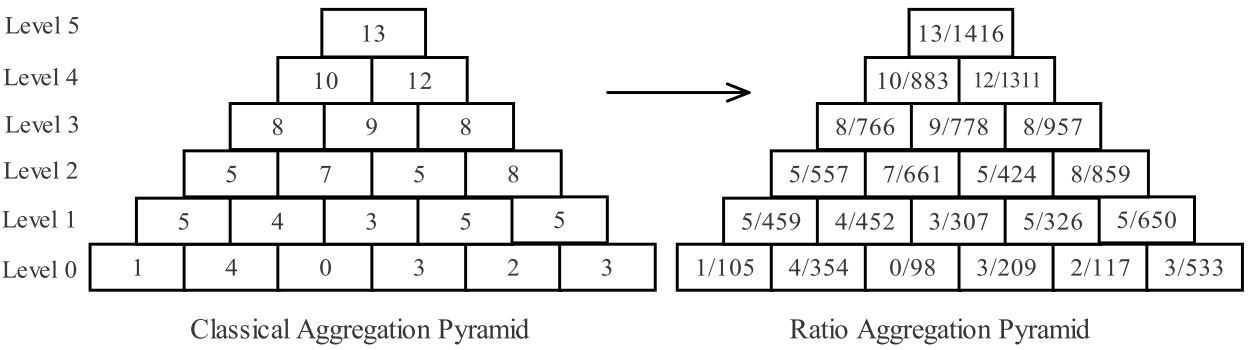
\includegraphics[height=4.4cm]{images/ratiopyramid.png}}
\caption{Von der klassischen 'Aggregataion Pyramid' zur 'Ratio Aggreation Pyramid' \cite{yuan2007online}}
\label{fig:ratiopyramid}
\end{figure*}


\begin{figure}[h]
    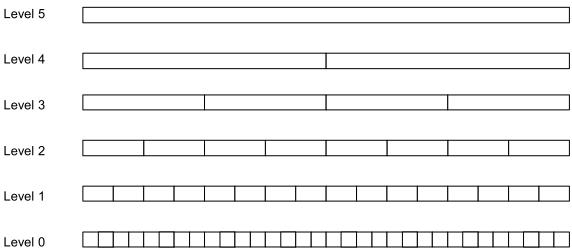
\includegraphics[width=.5\textwidth]{images/wavelet.jpg}
    \caption{Wavelet Tree \cite{Zhu:2003:EEB:956750.956789}}
    \label{fig:wavelet}
\end{figure}

Eine spezielles Modell entwickeln Zhu et. al. in 'Efficient Elastic Burst Detection in Data Streams' \cite{Zhu:2003:EEB:956750.956789} mit dem Elastic Window, bei dem   die Größe der Zeitfenster variiert. Somit können die Bursts dynamischer durch deren Characterisik und unabhäniger von ihrer Dauer erkannt werden, die oftmals nicht im Vorfeld festgelegt werden kann. Dafür wird ein Wavelet-Tree vom Stream erzeugt, bei dem die Wavelet-Kooefizienten den Aggregaten der Fenster entsprechen. Wie in Abbildung \ref{wavelet} zu sehen ist, wird zu Beginn der Stream in Fenster unterteilt, die disjunkt nebeneinander liegen. Je Fenster wird ein Aggregat erstellt, in der Regel werden dazu die Ergeinisse eines bestimmten Typs oder mit gleichen Attributen gezählt. Diese Aggreagte bilden nun selbst wiederum einen Stream. Das Verfahren wird wiederholt, vorrausgesetzt es befinden sich entsprechende Ereignisse bzw. Aggregierte Ereignisse im Stream. Mit jedem Schritt wird der betrachtete Zeitabschnitt größer und man bewegt in das nächst höhere Level Richtung Wurzel des Baums. Zu jedem Level wird ein Schwellwert angegeben, bei dessen Überscheitung ein Burst ausgelöst wird.

\begin{figure*}[htbp]
\centerline{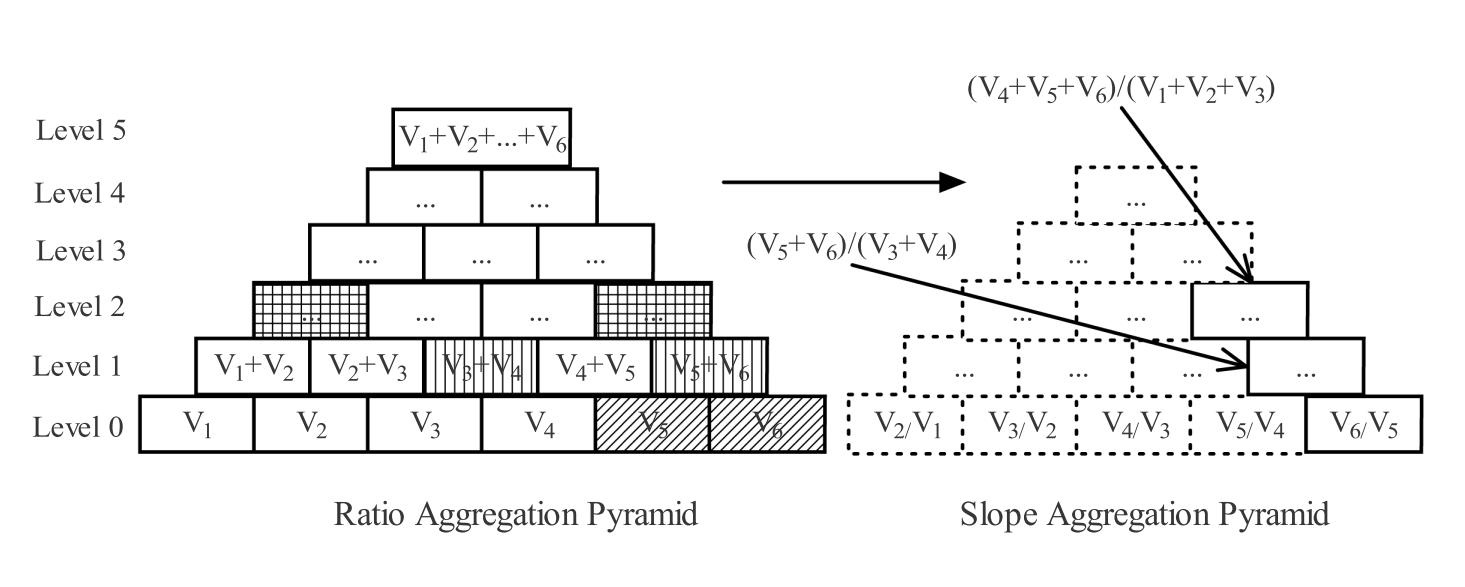
\includegraphics[height=6.3cm]{images/slopepyramid.jpg}}
\caption{Berechnungsbeispiel zur 'Slope Pyramid' \cite{yuan2007online}}
\label{fig:slopepyramid}
\end{figure*}

% \begin{figure*}
%     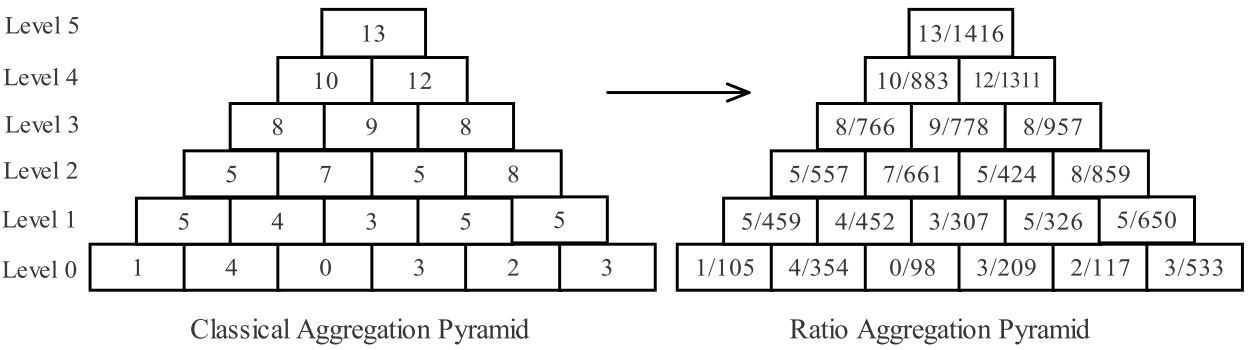
\includegraphics[width.5=\textwidth]{images/ratiopyramid.jpg}
%     \caption{Von der klassischen 'Aggregataion Pyramid' zur 'Ratio Aggreation Pyramid' \cite{yuan2007online}}
%     \label{fig:ratiopyramid}
% \end{figure*}



Yuan et. al. entwickeln in 'Online Burst Detection Over High Speed Short Text Streams' \cite{yuan2007online} ein Verfahren das auf einem Wavelet-Tree basiert. Dieser kann auch als Pyarmide betratchtet werden, mit den Levels die dem Aggregierungsgrad entsprechen. Da die Burst-Detection sich auf den Schwellwert des jeweiligen Lebels stützt, muss dieser zu beginnder Analyse feststehen. Das kann eine Herrausforderung sein, denn damit muss auch die Menge an Ereignissen im Stream eingeschätzt werden können. Um diese Problem zu lösen werden keine Absoluten Angaben der Aggregatewerte verwendet, wie zum Beispiel deren Anzahl. Stattdessen wird angegeben, wieviele relevante Events aggregiert wurden im Verhältnis zu allen aufgetretenen Events im betroffenen Zeitraum. Abbildung \ref{fig:ratiopyramid}. Eine weitere Komprimierung wird durch die Slope Pyarmid, wie in Abbildung \ref{fig:slopepyramid} dargestellt, erreicht. Dabei wird der Fokus auf die Veränderung von Fenster zu Fenster gelegt. Dazu wird Verhältniswert aus der Ratio Pyamid herangezogen; der Wert des vorhegehenden Fensters wird mit dem des aktuellen Fenster dividiert.\cite{yuan2007online}\\

Besondere Anforderungen stellt die Realtime-Burst Detection in Verbindung mit der gleichzeitigen Betrachtung mehrerer Fenstergrößen. Übliche Burst-Detektionsverfahren sind für eine Echtzeiterkennung nicht schnell genug, daher wurde von Ebina et. al. \cite{ebina2011real}  Burst-Erkennungsmethode weiter entwickelt. Das Ziel ist dabei die Berechnungszeit zu reduzieren, indem redundante Datenaktualisierungen wie bei Yuan et. al. vermieden werden. Dazu werden  die letzen Zellen der Slope Pyarmid auf effizientere Weise berechnet.\cite{ebina2011real}\\

Je nach Use Case sind auch aufwändigere Analysen wie in 'Event Detection with Burst Information Networks' \cite{ge2016event} notwendig.

% Detecting ‘bursts’ in time series data with Kleinberg’s burst detection algorithm
% \cite{kleinberg1}

\subsection{Social Media Analyse}
Eine ganze Reihe von Arbeiten beschäftigt sich mit der Analyse der Aktivitäten der Wikipedia-Nutzer.

\begin{itemize}
\item Extracting Event-Related Information from Article Updates in Wikipedia \cite{10.1007978-3-642-36973-5_22}
\item Ongoing events in Wikipedia: a cross-lingual case study \cite{gottschalk2017ongoing}
\item How much is Wikipedia Lagging Behind News? \cite{fetahu2015much}
\item Event analysis in social multimedia: a survey \cite{liu2016event}
\item A cloud-enabled automatic disaster analysis system of multi-sourced data streams: An example synthesizing social media, remote sensing and Wikipedia data \cite{huang2017cloud}
\end{itemize}

% Des weiteren 

% Pinterest
% I need to try this?: a statistical overview of pinterest
% \cite{gilbert2013need}

% Twitter
% An evaluation of the run-time and task-based performance of event detection techniques for Twitter
% \cite{weiler2016evaluation}
